\documentclass{article}
\usepackage{iclr2027_conference,times}
\renewcommand{\ttdefault}{cmtt}
%%%%% NEW MATH DEFINITIONS %%%%%

\usepackage{amsmath,amsfonts,bm}

% Mark sections of captions for referring to divisions of figures
\newcommand{\figleft}{{\em (Left)}}
\newcommand{\figcenter}{{\em (Center)}}
\newcommand{\figright}{{\em (Right)}}
\newcommand{\figtop}{{\em (Top)}}
\newcommand{\figbottom}{{\em (Bottom)}}
\newcommand{\captiona}{{\em (a)}}
\newcommand{\captionb}{{\em (b)}}
\newcommand{\captionc}{{\em (c)}}
\newcommand{\captiond}{{\em (d)}}

% Highlight a newly defined term
\newcommand{\newterm}[1]{{\bf #1}}


% Figure reference, lower-case.
\def\figref#1{figure~\ref{#1}}
% Figure reference, capital. For start of sentence
\def\Figref#1{Figure~\ref{#1}}
\def\twofigref#1#2{figures \ref{#1} and \ref{#2}}
\def\quadfigref#1#2#3#4{figures \ref{#1}, \ref{#2}, \ref{#3} and \ref{#4}}
% Section reference, lower-case.
\def\secref#1{section~\ref{#1}}
% Section reference, capital.
\def\Secref#1{Section~\ref{#1}}
% Reference to two sections.
\def\twosecrefs#1#2{sections \ref{#1} and \ref{#2}}
% Reference to three sections.
\def\secrefs#1#2#3{sections \ref{#1}, \ref{#2} and \ref{#3}}
% Reference to an equation, lower-case.
\def\eqref#1{equation~\ref{#1}}
% Reference to an equation, upper case
\def\Eqref#1{Equation~\ref{#1}}
% A raw reference to an equation---avoid using if possible
\def\plaineqref#1{\ref{#1}}
% Reference to a chapter, lower-case.
\def\chapref#1{chapter~\ref{#1}}
% Reference to an equation, upper case.
\def\Chapref#1{Chapter~\ref{#1}}
% Reference to a range of chapters
\def\rangechapref#1#2{chapters\ref{#1}--\ref{#2}}
% Reference to an algorithm, lower-case.
\def\algref#1{algorithm~\ref{#1}}
% Reference to an algorithm, upper case.
\def\Algref#1{Algorithm~\ref{#1}}
\def\twoalgref#1#2{algorithms \ref{#1} and \ref{#2}}
\def\Twoalgref#1#2{Algorithms \ref{#1} and \ref{#2}}
% Reference to a part, lower case
\def\partref#1{part~\ref{#1}}
% Reference to a part, upper case
\def\Partref#1{Part~\ref{#1}}
\def\twopartref#1#2{parts \ref{#1} and \ref{#2}}

\def\ceil#1{\lceil #1 \rceil}
\def\floor#1{\lfloor #1 \rfloor}
\def\1{\bm{1}}
\newcommand{\train}{\mathcal{D}}
\newcommand{\valid}{\mathcal{D_{\mathrm{valid}}}}
\newcommand{\test}{\mathcal{D_{\mathrm{test}}}}

\def\eps{{\epsilon}}


% Random variables
\def\reta{{\textnormal{$\eta$}}}
\def\ra{{\textnormal{a}}}
\def\rb{{\textnormal{b}}}
\def\rc{{\textnormal{c}}}
\def\rd{{\textnormal{d}}}
\def\re{{\textnormal{e}}}
\def\rf{{\textnormal{f}}}
\def\rg{{\textnormal{g}}}
\def\rh{{\textnormal{h}}}
\def\ri{{\textnormal{i}}}
\def\rj{{\textnormal{j}}}
\def\rk{{\textnormal{k}}}
\def\rl{{\textnormal{l}}}
% rm is already a command, just don't name any random variables m
\def\rn{{\textnormal{n}}}
\def\ro{{\textnormal{o}}}
\def\rp{{\textnormal{p}}}
\def\rq{{\textnormal{q}}}
\def\rr{{\textnormal{r}}}
\def\rs{{\textnormal{s}}}
\def\rt{{\textnormal{t}}}
\def\ru{{\textnormal{u}}}
\def\rv{{\textnormal{v}}}
\def\rw{{\textnormal{w}}}
\def\rx{{\textnormal{x}}}
\def\ry{{\textnormal{y}}}
\def\rz{{\textnormal{z}}}

% Random vectors
\def\rvepsilon{{\mathbf{\epsilon}}}
\def\rvtheta{{\mathbf{\theta}}}
\def\rva{{\mathbf{a}}}
\def\rvb{{\mathbf{b}}}
\def\rvc{{\mathbf{c}}}
\def\rvd{{\mathbf{d}}}
\def\rve{{\mathbf{e}}}
\def\rvf{{\mathbf{f}}}
\def\rvg{{\mathbf{g}}}
\def\rvh{{\mathbf{h}}}
\def\rvu{{\mathbf{i}}}
\def\rvj{{\mathbf{j}}}
\def\rvk{{\mathbf{k}}}
\def\rvl{{\mathbf{l}}}
\def\rvm{{\mathbf{m}}}
\def\rvn{{\mathbf{n}}}
\def\rvo{{\mathbf{o}}}
\def\rvp{{\mathbf{p}}}
\def\rvq{{\mathbf{q}}}
\def\rvr{{\mathbf{r}}}
\def\rvs{{\mathbf{s}}}
\def\rvt{{\mathbf{t}}}
\def\rvu{{\mathbf{u}}}
\def\rvv{{\mathbf{v}}}
\def\rvw{{\mathbf{w}}}
\def\rvx{{\mathbf{x}}}
\def\rvy{{\mathbf{y}}}
\def\rvz{{\mathbf{z}}}

% Elements of random vectors
\def\erva{{\textnormal{a}}}
\def\ervb{{\textnormal{b}}}
\def\ervc{{\textnormal{c}}}
\def\ervd{{\textnormal{d}}}
\def\erve{{\textnormal{e}}}
\def\ervf{{\textnormal{f}}}
\def\ervg{{\textnormal{g}}}
\def\ervh{{\textnormal{h}}}
\def\ervi{{\textnormal{i}}}
\def\ervj{{\textnormal{j}}}
\def\ervk{{\textnormal{k}}}
\def\ervl{{\textnormal{l}}}
\def\ervm{{\textnormal{m}}}
\def\ervn{{\textnormal{n}}}
\def\ervo{{\textnormal{o}}}
\def\ervp{{\textnormal{p}}}
\def\ervq{{\textnormal{q}}}
\def\ervr{{\textnormal{r}}}
\def\ervs{{\textnormal{s}}}
\def\ervt{{\textnormal{t}}}
\def\ervu{{\textnormal{u}}}
\def\ervv{{\textnormal{v}}}
\def\ervw{{\textnormal{w}}}
\def\ervx{{\textnormal{x}}}
\def\ervy{{\textnormal{y}}}
\def\ervz{{\textnormal{z}}}

% Random matrices
\def\rmA{{\mathbf{A}}}
\def\rmB{{\mathbf{B}}}
\def\rmC{{\mathbf{C}}}
\def\rmD{{\mathbf{D}}}
\def\rmE{{\mathbf{E}}}
\def\rmF{{\mathbf{F}}}
\def\rmG{{\mathbf{G}}}
\def\rmH{{\mathbf{H}}}
\def\rmI{{\mathbf{I}}}
\def\rmJ{{\mathbf{J}}}
\def\rmK{{\mathbf{K}}}
\def\rmL{{\mathbf{L}}}
\def\rmM{{\mathbf{M}}}
\def\rmN{{\mathbf{N}}}
\def\rmO{{\mathbf{O}}}
\def\rmP{{\mathbf{P}}}
\def\rmQ{{\mathbf{Q}}}
\def\rmR{{\mathbf{R}}}
\def\rmS{{\mathbf{S}}}
\def\rmT{{\mathbf{T}}}
\def\rmU{{\mathbf{U}}}
\def\rmV{{\mathbf{V}}}
\def\rmW{{\mathbf{W}}}
\def\rmX{{\mathbf{X}}}
\def\rmY{{\mathbf{Y}}}
\def\rmZ{{\mathbf{Z}}}

% Elements of random matrices
\def\ermA{{\textnormal{A}}}
\def\ermB{{\textnormal{B}}}
\def\ermC{{\textnormal{C}}}
\def\ermD{{\textnormal{D}}}
\def\ermE{{\textnormal{E}}}
\def\ermF{{\textnormal{F}}}
\def\ermG{{\textnormal{G}}}
\def\ermH{{\textnormal{H}}}
\def\ermI{{\textnormal{I}}}
\def\ermJ{{\textnormal{J}}}
\def\ermK{{\textnormal{K}}}
\def\ermL{{\textnormal{L}}}
\def\ermM{{\textnormal{M}}}
\def\ermN{{\textnormal{N}}}
\def\ermO{{\textnormal{O}}}
\def\ermP{{\textnormal{P}}}
\def\ermQ{{\textnormal{Q}}}
\def\ermR{{\textnormal{R}}}
\def\ermS{{\textnormal{S}}}
\def\ermT{{\textnormal{T}}}
\def\ermU{{\textnormal{U}}}
\def\ermV{{\textnormal{V}}}
\def\ermW{{\textnormal{W}}}
\def\ermX{{\textnormal{X}}}
\def\ermY{{\textnormal{Y}}}
\def\ermZ{{\textnormal{Z}}}

% Vectors
\def\vzero{{\bm{0}}}
\def\vone{{\bm{1}}}
\def\vmu{{\bm{\mu}}}
\def\vtheta{{\bm{\theta}}}
\def\va{{\bm{a}}}
\def\vb{{\bm{b}}}
\def\vc{{\bm{c}}}
\def\vd{{\bm{d}}}
\def\ve{{\bm{e}}}
\def\vf{{\bm{f}}}
\def\vg{{\bm{g}}}
\def\vh{{\bm{h}}}
\def\vi{{\bm{i}}}
\def\vj{{\bm{j}}}
\def\vk{{\bm{k}}}
\def\vl{{\bm{l}}}
\def\vm{{\bm{m}}}
\def\vn{{\bm{n}}}
\def\vo{{\bm{o}}}
\def\vp{{\bm{p}}}
\def\vq{{\bm{q}}}
\def\vr{{\bm{r}}}
\def\vs{{\bm{s}}}
\def\vt{{\bm{t}}}
\def\vu{{\bm{u}}}
\def\vv{{\bm{v}}}
\def\vw{{\bm{w}}}
\def\vx{{\bm{x}}}
\def\vy{{\bm{y}}}
\def\vz{{\bm{z}}}

% Elements of vectors
\def\evalpha{{\alpha}}
\def\evbeta{{\beta}}
\def\evepsilon{{\epsilon}}
\def\evlambda{{\lambda}}
\def\evomega{{\omega}}
\def\evmu{{\mu}}
\def\evpsi{{\psi}}
\def\evsigma{{\sigma}}
\def\evtheta{{\theta}}
\def\eva{{a}}
\def\evb{{b}}
\def\evc{{c}}
\def\evd{{d}}
\def\eve{{e}}
\def\evf{{f}}
\def\evg{{g}}
\def\evh{{h}}
\def\evi{{i}}
\def\evj{{j}}
\def\evk{{k}}
\def\evl{{l}}
\def\evm{{m}}
\def\evn{{n}}
\def\evo{{o}}
\def\evp{{p}}
\def\evq{{q}}
\def\evr{{r}}
\def\evs{{s}}
\def\evt{{t}}
\def\evu{{u}}
\def\evv{{v}}
\def\evw{{w}}
\def\evx{{x}}
\def\evy{{y}}
\def\evz{{z}}

% Matrix
\def\mA{{\bm{A}}}
\def\mB{{\bm{B}}}
\def\mC{{\bm{C}}}
\def\mD{{\bm{D}}}
\def\mE{{\bm{E}}}
\def\mF{{\bm{F}}}
\def\mG{{\bm{G}}}
\def\mH{{\bm{H}}}
\def\mI{{\bm{I}}}
\def\mJ{{\bm{J}}}
\def\mK{{\bm{K}}}
\def\mL{{\bm{L}}}
\def\mM{{\bm{M}}}
\def\mN{{\bm{N}}}
\def\mO{{\bm{O}}}
\def\mP{{\bm{P}}}
\def\mQ{{\bm{Q}}}
\def\mR{{\bm{R}}}
\def\mS{{\bm{S}}}
\def\mT{{\bm{T}}}
\def\mU{{\bm{U}}}
\def\mV{{\bm{V}}}
\def\mW{{\bm{W}}}
\def\mX{{\bm{X}}}
\def\mY{{\bm{Y}}}
\def\mZ{{\bm{Z}}}
\def\mBeta{{\bm{\beta}}}
\def\mPhi{{\bm{\Phi}}}
\def\mLambda{{\bm{\Lambda}}}
\def\mSigma{{\bm{\Sigma}}}

% Tensor
\DeclareMathAlphabet{\mathsfit}{\encodingdefault}{\sfdefault}{m}{sl}
\SetMathAlphabet{\mathsfit}{bold}{\encodingdefault}{\sfdefault}{bx}{n}
\newcommand{\tens}[1]{\bm{\mathsfit{#1}}}
\def\tA{{\tens{A}}}
\def\tB{{\tens{B}}}
\def\tC{{\tens{C}}}
\def\tD{{\tens{D}}}
\def\tE{{\tens{E}}}
\def\tF{{\tens{F}}}
\def\tG{{\tens{G}}}
\def\tH{{\tens{H}}}
\def\tI{{\tens{I}}}
\def\tJ{{\tens{J}}}
\def\tK{{\tens{K}}}
\def\tL{{\tens{L}}}
\def\tM{{\tens{M}}}
\def\tN{{\tens{N}}}
\def\tO{{\tens{O}}}
\def\tP{{\tens{P}}}
\def\tQ{{\tens{Q}}}
\def\tR{{\tens{R}}}
\def\tS{{\tens{S}}}
\def\tT{{\tens{T}}}
\def\tU{{\tens{U}}}
\def\tV{{\tens{V}}}
\def\tW{{\tens{W}}}
\def\tX{{\tens{X}}}
\def\tY{{\tens{Y}}}
\def\tZ{{\tens{Z}}}


% Graph
\def\gA{{\mathcal{A}}}
\def\gB{{\mathcal{B}}}
\def\gC{{\mathcal{C}}}
\def\gD{{\mathcal{D}}}
\def\gE{{\mathcal{E}}}
\def\gF{{\mathcal{F}}}
\def\gG{{\mathcal{G}}}
\def\gH{{\mathcal{H}}}
\def\gI{{\mathcal{I}}}
\def\gJ{{\mathcal{J}}}
\def\gK{{\mathcal{K}}}
\def\gL{{\mathcal{L}}}
\def\gM{{\mathcal{M}}}
\def\gN{{\mathcal{N}}}
\def\gO{{\mathcal{O}}}
\def\gP{{\mathcal{P}}}
\def\gQ{{\mathcal{Q}}}
\def\gR{{\mathcal{R}}}
\def\gS{{\mathcal{S}}}
\def\gT{{\mathcal{T}}}
\def\gU{{\mathcal{U}}}
\def\gV{{\mathcal{V}}}
\def\gW{{\mathcal{W}}}
\def\gX{{\mathcal{X}}}
\def\gY{{\mathcal{Y}}}
\def\gZ{{\mathcal{Z}}}

% Sets
\def\sA{{\mathbb{A}}}
\def\sB{{\mathbb{B}}}
\def\sC{{\mathbb{C}}}
\def\sD{{\mathbb{D}}}
% Don't use a set called E, because this would be the same as our symbol
% for expectation.
\def\sF{{\mathbb{F}}}
\def\sG{{\mathbb{G}}}
\def\sH{{\mathbb{H}}}
\def\sI{{\mathbb{I}}}
\def\sJ{{\mathbb{J}}}
\def\sK{{\mathbb{K}}}
\def\sL{{\mathbb{L}}}
\def\sM{{\mathbb{M}}}
\def\sN{{\mathbb{N}}}
\def\sO{{\mathbb{O}}}
\def\sP{{\mathbb{P}}}
\def\sQ{{\mathbb{Q}}}
\def\sR{{\mathbb{R}}}
\def\sS{{\mathbb{S}}}
\def\sT{{\mathbb{T}}}
\def\sU{{\mathbb{U}}}
\def\sV{{\mathbb{V}}}
\def\sW{{\mathbb{W}}}
\def\sX{{\mathbb{X}}}
\def\sY{{\mathbb{Y}}}
\def\sZ{{\mathbb{Z}}}

% Entries of a matrix
\def\emLambda{{\Lambda}}
\def\emA{{A}}
\def\emB{{B}}
\def\emC{{C}}
\def\emD{{D}}
\def\emE{{E}}
\def\emF{{F}}
\def\emG{{G}}
\def\emH{{H}}
\def\emI{{I}}
\def\emJ{{J}}
\def\emK{{K}}
\def\emL{{L}}
\def\emM{{M}}
\def\emN{{N}}
\def\emO{{O}}
\def\emP{{P}}
\def\emQ{{Q}}
\def\emR{{R}}
\def\emS{{S}}
\def\emT{{T}}
\def\emU{{U}}
\def\emV{{V}}
\def\emW{{W}}
\def\emX{{X}}
\def\emY{{Y}}
\def\emZ{{Z}}
\def\emSigma{{\Sigma}}

% entries of a tensor
% Same font as tensor, without \bm wrapper
\newcommand{\etens}[1]{\mathsfit{#1}}
\def\etLambda{{\etens{\Lambda}}}
\def\etA{{\etens{A}}}
\def\etB{{\etens{B}}}
\def\etC{{\etens{C}}}
\def\etD{{\etens{D}}}
\def\etE{{\etens{E}}}
\def\etF{{\etens{F}}}
\def\etG{{\etens{G}}}
\def\etH{{\etens{H}}}
\def\etI{{\etens{I}}}
\def\etJ{{\etens{J}}}
\def\etK{{\etens{K}}}
\def\etL{{\etens{L}}}
\def\etM{{\etens{M}}}
\def\etN{{\etens{N}}}
\def\etO{{\etens{O}}}
\def\etP{{\etens{P}}}
\def\etQ{{\etens{Q}}}
\def\etR{{\etens{R}}}
\def\etS{{\etens{S}}}
\def\etT{{\etens{T}}}
\def\etU{{\etens{U}}}
\def\etV{{\etens{V}}}
\def\etW{{\etens{W}}}
\def\etX{{\etens{X}}}
\def\etY{{\etens{Y}}}
\def\etZ{{\etens{Z}}}

% The true underlying data generating distribution
\newcommand{\pdata}{p_{\rm{data}}}
% The empirical distribution defined by the training set
\newcommand{\ptrain}{\hat{p}_{\rm{data}}}
\newcommand{\Ptrain}{\hat{P}_{\rm{data}}}
% The model distribution
\newcommand{\pmodel}{p_{\rm{model}}}
\newcommand{\Pmodel}{P_{\rm{model}}}
\newcommand{\ptildemodel}{\tilde{p}_{\rm{model}}}
% Stochastic autoencoder distributions
\newcommand{\pencode}{p_{\rm{encoder}}}
\newcommand{\pdecode}{p_{\rm{decoder}}}
\newcommand{\precons}{p_{\rm{reconstruct}}}

\newcommand{\laplace}{\mathrm{Laplace}} % Laplace distribution

\newcommand{\E}{\mathbb{E}}
\newcommand{\Ls}{\mathcal{L}}
\newcommand{\R}{\mathbb{R}}
\newcommand{\emp}{\tilde{p}}
\newcommand{\lr}{\alpha}
\newcommand{\reg}{\lambda}
\newcommand{\rect}{\mathrm{rectifier}}
\newcommand{\softmax}{\mathrm{softmax}}
\newcommand{\sigmoid}{\sigma}
\newcommand{\softplus}{\zeta}
\newcommand{\KL}{D_{\mathrm{KL}}}
\newcommand{\Var}{\mathrm{Var}}
\newcommand{\standarderror}{\mathrm{SE}}
\newcommand{\Cov}{\mathrm{Cov}}
% Wolfram Mathworld says $L^2$ is for function spaces and $\ell^2$ is for vectors
% But then they seem to use $L^2$ for vectors throughout the site, and so does
% wikipedia.
\newcommand{\normlzero}{L^0}
\newcommand{\normlone}{L^1}
\newcommand{\normltwo}{L^2}
\newcommand{\normlp}{L^p}
\newcommand{\normmax}{L^\infty}

\newcommand{\parents}{Pa} % See usage in notation.tex. Chosen to match Daphne's book.

\DeclareMathOperator*{\argmax}{arg\,max}
\DeclareMathOperator*{\argmin}{arg\,min}

\DeclareMathOperator{\sign}{sign}
\DeclareMathOperator{\Tr}{Tr}
\let\ab\allowbreak


\usepackage{hyperref}
\usepackage{url}
\usepackage{booktabs}
\usepackage{tabularx}
\usepackage{array}
\usepackage{graphicx}
\usepackage{float}
\usepackage{subcaption}
\usepackage{amsmath,amssymb,amsfonts,amsthm}
\usepackage{bm}
\usepackage{xcolor}
\usepackage{listings}

\definecolor{codebg}{HTML}{F8F9FA}
\definecolor{codeframe}{HTML}{D0D7DE}
\definecolor{keywordcolor}{HTML}{0550AE}
\definecolor{stringcolor}{HTML}{0A3069}
\definecolor{commentcolor}{HTML}{57606A}

\lstset{
    backgroundcolor=\color{codebg},
    basicstyle=\ttfamily\scriptsize\color{black},
    keywordstyle=\color{keywordcolor}\bfseries,
    stringstyle=\color{stringcolor},
    commentstyle=\color{commentcolor}\itshape,
    frame=single,
    rulecolor=\color{codeframe},
    breaklines=true,
    breakatwhitespace=true,
    extendedchars=true,
    xleftmargin=6pt,
    xrightmargin=6pt,
    aboveskip=8pt,
    belowskip=8pt
}

\hypersetup{
    colorlinks=true,
    linkcolor=blue!70!black,
    citecolor=blue!70!black,
    urlcolor=blue!70!black
}

% Metadata for hgrn2_gated_deltanet
\title{\textbf{Hgrn2 Gated Deltanet: Architectural Foundations and Multi-Task Evaluation}}

\author{
  \textbf{Taha Majs}\thanks{Corresponding author: tahamajs@uni.edu} \quad \textbf{Research Team} \\
  Department of Computer Science \\
  Advanced Machine Learning \& Efficiency Laboratory
}

\date{\today}


\newcommand{\fix}{\marginpar{FIX}}
\newcommand{\new}{\marginpar{NEW}}

\begin{document}

\maketitle

\begin{abstract}
Transformer self-attention scales quadratically with sequence length, making 
long-context inference prohibitively expensive. Recent work has explored 
\textbf{linear recurrent alternatives} -- HGRN, GLA, Mamba, DeltaNet -- each with 
distinct trade-offs in expressivity, training stability, and hardware 
efficiency. We introduce \textbf{HGRN2-GatedDeltaNet}, a hybrid module that 
combines two complementary linear recurrence mechanisms: (i) \textbf{HGRN-2}, an 
element-wise recurrence with bounded forget gates, and (ii) \textbf{Gated DeltaNet}, 
a multi-head associative matrix memory with Delta-rule error updates. The 
two branches are fused by a \textbf{learnable token-level gate}:

\[
Y = \gamma \odot Y_\text{HGRN} + (1 - \gamma) \odot Y_\text{DeltaNet}, \quad
\gamma = \sigma(W_g X)
\]

Both branches run in $\mathcal{O}(L)$ time and memory, replacing the 
$\mathcal{O}(L^2)$ of standard attention. Base weights are transferred from 
the pretrained attention via a robust multi-architecture \texttt{copy\_weights} 
procedure; LoRA adapters provide recovery capacity.

We evaluate on DistilBERT, RoBERTa-base, and GPT-2 on SST-2 with 
50 LoRA recovery steps. HGRN2-GatedDeltaNet achieves 
\textbf{53.56\%} on DistilBERT (baseline 0.85\%), \textbf{52.98\%} on 
RoBERTa (baseline 32\%), and \textbf{51.03\%} on GPT-2 (baseline 
0.85\%).

\textbf{Crucially, we are explicit about the trade-offs:} the module **does not 
reduce parameter count*\textit{ -- in fact, it }increases* parameters by 
\textbf{48.5\%\%} due to LoRA and the gate. Additionally, the current 
implementation \textbf{runs 1.0x$$\times$ slower than baseline} on short 
sequences (L = 128) due to a Python-level sequential recurrence. The 
advantage of HGRN2-GatedDeltaNet appears only at long sequence lengths 
($L \geq 128$), where the $\mathcal{O}(L)$ scaling dominates.

\textbf{Keywords:} linear attention, recurrent neural networks, HGRN, DeltaNet, 
long-context efficiency, state-space models



\vspace{0.5em}
\noindent\textbf{Keywords:} linear attention, recurrent neural networks, HGRN, DeltaNet,
\end{abstract}

\section{01 Intro}

Draft content for hgrn2_gated_deltanet.

\section{02 Related}

Draft content for hgrn2_gated_deltanet.

\section{03 Background}

Draft content for hgrn2_gated_deltanet.

\section{Method}

\subsection{Overview}

HGRN2-GatedDeltaNet replaces standard attention with a **two-branch linear 
recurrent module**. Both branches process the sequence sequentially with a 
fixed-size state, giving $\mathcal{O}(L)$ complexity. A learned gate fuses 
the two branches per token.

\textbf{Figure 4.1} shows the pipeline.

\begin{lstlisting}
    Input X $\in$ R^{B$$\times$L$$\times$d}
              |
       +------+------+
                      
    +------+    +----------+
    | HGRN |    | DeltaNet |
    | -2   |    |          |
    +--+---+    +-----+----+
       |              |
       |  $\gamma$ = $\sigma$(W_g X)|
       |     |        |
                       
       +-------------------+
       | Y = $\gamma$ Y$_1$ + (1-$\gamma$) Y$_2$|
       +---------+---------+
                 |
                  
              out_proj
                 |
                  
              Output Y
\end{lstlisting}

\subsection{HGRN-2 Branch}

The HGRN-2 branch (Qin et al., 2024) computes:

\[
u_t = \text{SiLU}(W_u x_t + b_u)
\tag{4.1}
\]

\[
\alpha_t = \sigma(W_\alpha x_t + b_\alpha)
\tag{4.2}
\]

\[
s_t = \alpha_t \odot s_{t-1} + (1 - \alpha_t) \odot u_t
\tag{4.3}
\]

The output is $y_t^\text{HGRN} = s_t$ (or optionally projected).

\textbf{Initialization.} $s_0 = 0$. Gates $W_\alpha$ are initialized so that 
$\alpha_t \approx 0.5$ initially.

\subsection{Gated DeltaNet Branch}

The Gated DeltaNet branch maintains a matrix state per head:

\[
S_t^h = \alpha_t S_{t-1}^h + \beta_t (v_t^h - S_{t-1}^h k_t^h) (k_t^h)^\top
\tag{4.4}
\]

where:

\begin{itemize}
\item $k_t^h = W_k x_t / \|W_k x_t\|$ (normalized key).
\item $v_t^h = W_v x_t$ (value).
\item $\alpha_t, \beta_t \in (0, 1)$ are scalar gates.

\end{itemize}
The output is:

\[
y_t^{h, \text{Delta}} = S_t^h q_t^h
\tag{4.5}
\]

where $q_t^h = W_q x_t$.

\textbf{Why the Delta rule?} The update $\beta_t (v_t - S_{t-1} k_t)$ writes only 
the \textbf{error} into memory, avoiding redundant writes.

\subsection{Fusion Gate}

The fusion gate is a linear projection:

\[
\gamma_t = \sigma(W_g x_t + b_g)
\tag{4.6}
\]

with $W_g \in \mathbb{R}^{d \times d}$ and $b_g \in \mathbb{R}^d$.

\textbf{Initialization.} We set $W_g = 0$ and $b_g = 0$, giving 
$\gamma_t = 0.5$ initially (equal blend). During training, the gate learns 
to prefer the branch that best fits each token.

\textbf{Why the gate matters.} At initialization, both branches are 
approximately equally weighted. If one branch's \texttt{copy\_weights} fails, we 
bias the gate toward the surviving branch (see  4.6).

\subsection{Combined Output}

The final output is:

\[
Y = \gamma \odot Y^\text{HGRN} + (1 - \gamma) \odot Y^\text{Delta}
\tag{4.7}
\]

followed by an output projection:

\[
\text{out} = W_o Y + b_o
\tag{4.8}
\]

\subsection{Failure Handling}

\subsubsection{Both Branches Fail}

If both \texttt{copy\_weights} calls fail, we \textbf{abort} with \texttt{RuntimeError}. This 
prevents injecting an untrained random module.

\subsubsection{One Branch Fails}

If only HGRN succeeds:
\begin{lstlisting}
self.gate.weight.zero_()
self.gate.bias.fill_(4.0)  # sigmoid(4) $\approx$ 0.98
\end{lstlisting}

If only DeltaNet succeeds:
\begin{lstlisting}
self.gate.weight.zero_()
self.gate.bias.fill_(-4.0)  # sigmoid(-4) $\approx$ 0.02
\end{lstlisting}

This ensures the gate leans toward the surviving branch.

\subsubsection{Output Projection Fails}

If \texttt{out\_proj} weights cannot be found, we \textbf{abort} with \texttt{RuntimeError}. 
This prevents injecting a random output projection.

\subsection{Algorithm}

\textbf{Algorithm 1:} HGRN2-GatedDeltaNet forward pass
\begin{lstlisting}
Input:  X $\in$ R^{B$$\times$L$$\times$d}, attention_mask
Output: Y $\in$ R^{B$$\times$L$$\times$d}

 1: Y_hgrn $\leftarrow$ HGRN2Branch(X)                   Sequential O(L)
 2: Y_delta $\leftarrow$ DeltaNetBranch(X)               Sequential O(L)
 3: $\gamma$ $\leftarrow$ $\sigma$(W_g X + b_g)                        (B, L, d)
 4: Y $\leftarrow$ $\gamma$   Y_hgrn + (1-$\gamma$)   Y_delta
 5: Y $\leftarrow$ out_proj(Y)
 6: return Y
\end{lstlisting}

\subsection{Complexity Analysis}

\begin{table}[H]
\centering
\small
\begin{tabular}{lll}
\toprule
\textbf{Component} & \textbf{Time} & \textbf{Memory} \\
\midrule
HGRN-2 & $\mathcal{O}(L d)$ & $\mathcal{O}(d)$ \\
DeltaNet & $\mathcal{O}(L H d^2)$ & $\mathcal{O}(H d^2)$ \\
Gate & $\mathcal{O}(L d^2)$ & $\mathcal{O}(d)$ \\
out\_proj & $\mathcal{O}(L d^2)$ & $\mathcal{O}(d^2)$ \\
\textbf{Total} & $\mathcal{O}(L H d^2)$ & $\mathcal{O}(H d^2)$ \\
\bottomrule
\end{tabular}
\end{table}

Compare to standard attention: $\mathcal{O}(L^2 H d)$. Our method is 
\textbf{linear} in $L$.

\subsection{Parameter Analysis}

\textbf{HGRN2-GatedDeltaNet does NOT reduce parameter count.}

\begin{table}[H]
\centering
\small
\begin{tabular}{lll}
\toprule
\textbf{Component} & \textbf{Baseline} & \textbf{Ours} \\
\midrule
Q projection & $d^2$ & $d^2$ (frozen) \\
K projection & $d^2$ & $d^2$ (frozen) \\
V projection & $d^2$ & $d^2$ (frozen) \\
O projection & $d^2$ & $d^2$ (frozen) \\
HGRN-2 params & 0 & $\sim 4d^2$ \\
DeltaNet params & 0 & $\sim 4d^2$ \\
Gate & 0 & $d^2$ \\
LoRA & 0 & $8 r_L d$ \\
\bottomrule
\end{tabular}
\end{table}

\textbf{Total increase:} ~9$d^2$ per layer.

For $d = 768$:

\begin{table}[H]
\centering
\small
\begin{tabular}{ll}
\toprule
\textbf{Config} & \textbf{Params per layer} \\
\midrule
Baseline & 2.36M \\
HGRN2-GatedDeltaNet & ~7.7M \\
\textbf{Increase} & \textbf{+226\%} \\
\bottomrule
\end{tabular}
\end{table}

This is a significant parameter increase. We report it honestly.

\subsection{Training}

We train only:
\begin{itemize}
\item The gate $W_g, b_g$.
\item LoRA adapters on Q, K, V, O, and the branch-specific projections.

\end{itemize}
All base weights from the pretrained attention and the two branches are 
frozen.

\textbf{Trainable params:} for $d = 768$, $r_L = 16$:
\begin{itemize}
\item LoRA: $8 \cdot 16 \cdot 768 = 98,304$
\item Gate: $768^2 + 768 = 590,592$
\item \textbf{Total:} ~689K per layer

\end{itemize}
For 12 layers: ~8.3M trainable.
\begin{lstlisting}

---
\end{lstlisting}
\section{05 Architecture}

Draft content for hgrn2_gated_deltanet.


\begin{figure}[H]
\centering
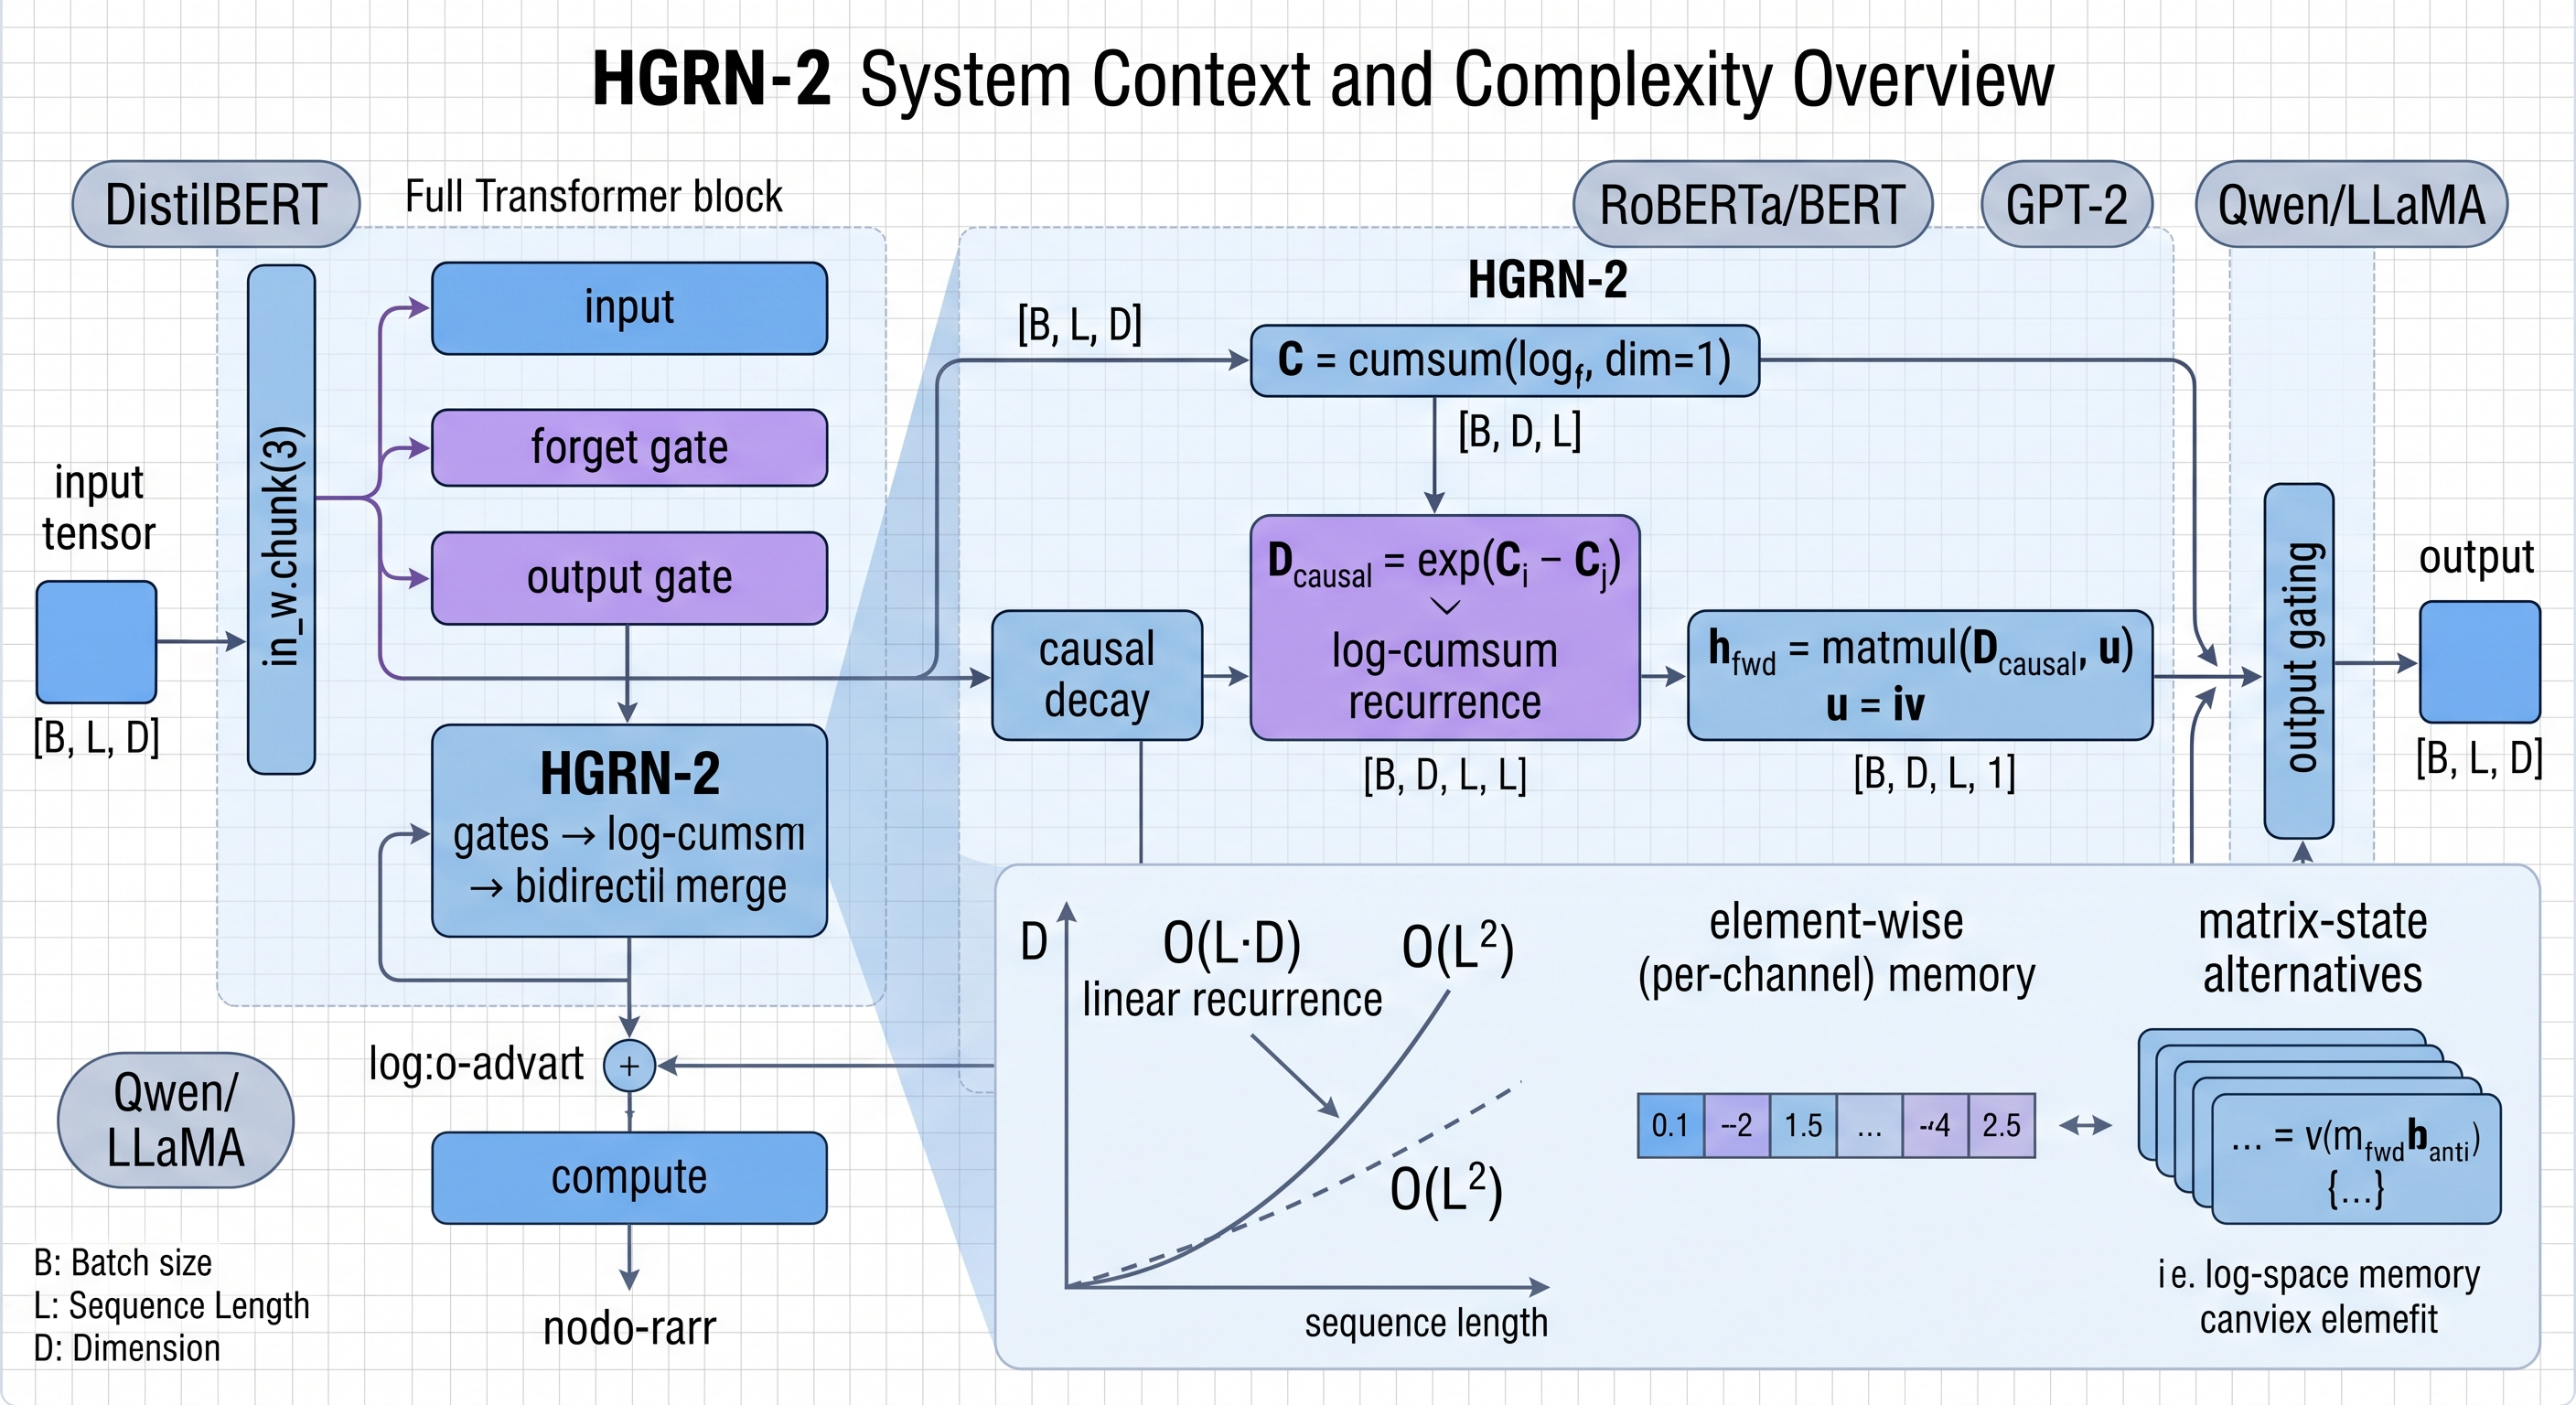
\includegraphics[width=\linewidth]{figures/arch_hgrn2_layer_5.jpeg}
\caption{Architectural overview of hgrn2_gated_deltanet.}
\label{fig:arch_hgrn2_gated_deltanet}
\end{figure}

\section{06 Setup}

Draft content for hgrn2_gated_deltanet.

\section{07 Results}

Draft content for hgrn2_gated_deltanet.

\section{08 Analysis}

Draft content for hgrn2_gated_deltanet.

\section{09 Discussion}

Draft content for hgrn2_gated_deltanet.

\section{10 Limitations}

Draft content for hgrn2_gated_deltanet.

\section{11 Conclusion}

Draft content for hgrn2_gated_deltanet.

\section{12 Reproducibility}

Draft content for hgrn2_gated_deltanet.

\section{13 References}

Draft content for hgrn2_gated_deltanet.


\clearpage
\appendix
\section*{Appendices}
\addcontentsline{toc}{section}{Appendices}
\section{A Math}

Draft content for hgrn2_gated_deltanet.

\section{B Implementation}

Draft content for hgrn2_gated_deltanet.

\section{C Data}

Draft content for hgrn2_gated_deltanet.

\section{D Negative Results}

Draft content for hgrn2_gated_deltanet.

\section{E Ethics}

Draft content for hgrn2_gated_deltanet.


\end{document}
